\section{Neo4J}

\subsection{Criação da base de dados}

\subsubsection{Motivação}

A base de dados grafica é ideal para as queries que relacionam muitas entidades entre si. Assim, poder-se-ia fazer o paralelismo com as queries que necessitam muitos Joins no modelo relacional.Isto é facilitado pelo fato da estrutura da base de dados ser um grafo.

\subsubsection{Criação - modificações}

Para a criaçao desta base de dados supôs-se a mesma aplicação que para o Mongo, ou seja, uma aplicação de procura de filmes por atores, categoria, etc e também para consultar as faturas dos clientes por loja, quem emitiu e onde.Dado a própria natureza do tipo de base de dados ainda conetou-se estas duas partes.

\subsection{Criação - Estrutura da Base de Dados}

A estrutura da base dados pode ser dividida em dois uma parte que relaciona os Filmes com os Atores, Categorias e Idiomas e outra que relaciona os Pagamentos com os Cliente,Lojas e os Staff.Assim pode-se identificar os seguintes nodos para a primeira parte:
\begin{itemize}

\item Filme: Representa um filme.Contem o identificador(id), o título(title), o ano em que o filme estreou(release\_year) e a descriçao do mesmo(description)
\hfill\\
\item Ator: Representa um ator que pode ter participado num Filme. Contem o identificador(id) do mesmo e o seu nome(name).
\hfill\\
\item Categoria: Representa uma categoria/género onde o Filme pode ser enquadrado. Contem o identificador e o nome da categoria(name)
\hfill\\
\item Idioma: Representa um dos idiomas que pode ser ouvidos os Filmes. Contem também o identificador (id) e a sua designação (name). 

\end{itemize}

Os relacionamentos para esta primeira "parte" são:

\begin{itemize}

\item Atuou\_Em: Relaciona os nodos Ator com os nodos Filme. Designa que atores participaram em que Filmes.
\hfill\\
\item Tem\_Categoria: Relaciona os nodos Filme com os nodos Categoria.Está relação permite estabelecer quais as Categorias a que o Filme pertence.
\hfill\\
\item Idioma\_Estrangeiro: Relaciona os nodos Filme com os nodos Idioma. Designa o Idioma estrangeiro em qual se pode ouvir o Filme.
\hfill\\
\item Idioma\_Original: Relaciona os nodos Filme com os nodos Idioma. Designa o Idioma original do Filme.No entanto, a relação não é usada visto que os dados que povoam a base dados MySQL não contem nenhuma entrada deste tipo.Apesar de estar no modelo lógico.
\end{itemize}

A segunda parte como foi mencionado diz respeito aos Pagamentos.Os nodos criados para representar esta situação foram os seguintes:

\begin{itemize}

\item Loja: Representa uma Loja onde se poderiam fazer aluguer de Filmes. Contem um identificador(id) e um identificador de manager(manager\_id). Para descobrir o nome do manager, por exemplo, cruza-se este identificador com os identificadores dos trabalhadores que estão nesta loja.
\hfill\\
\item Staff: Representa os trabalhadores das Lojas. Contem um identificador(id), o nome completo do mesmo (name) e o email (email).
\hfill\\
\item Cliente: Representa um cliente que já tenha feito algúm tipo de pagamento em umas das lojas. Contem um identificador do Cliente(id), o nome(name) e o email dele (email).
\hfill\\
\item Pagamento: Representa um pagamento realizado por um Cliente. Contem um identificador do Pagamento(id), a quantia que foi paga (amount) e a data em que foi realizado o mesmo (date).

\end{itemize}

Estes nodos são interligados com os seguintes relacionamentos:

\begin{itemize}

\item Trabalha\_Em : Relaciona os nodos Staff com os nodos Loja. Designa que trabalhadores estão a trabalhar em que Loja.
\hfill\\
\item Pertence : Relaciona os nodos Pagamento com os nodos Clientes. Designa os Pagamentos que foram efetuados pelo /Pertencem ao Cliente.
\hfill\\
\item Emitida\_Em : Relaciona os nodos Pagamento com os nodos Loja. Vinculando os Pagamentos as Lojas onde foram efetuadas.
\hfill\\
\item Emitida\_Por : Relaciona os nodos Pagamentos com os nodos Staff. Vincula os pagamentos com que os emitiu.

\end{itemize}

Nas seguintes imagem encontra-se uma representação gráfica dos nodos e relacionamentos mencionados acima. Sendo a primeira imagem da primeira parte e segunda  da segunda parte.

\begin{figure}[H]

  \centering

  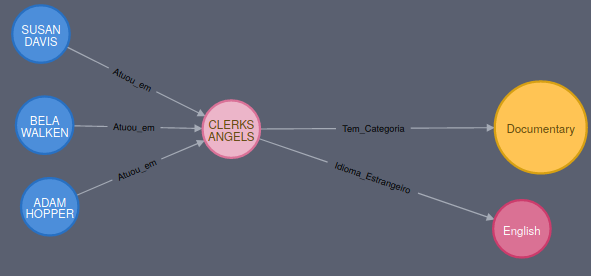
\includegraphics[width=\textwidth]{Movie.png}

  \caption {Representação gráfica dos nodos e Relacionamentos dos Filmes}

  \label {fig:Filme}

\end{figure}


\begin{figure}[H]

  \centering

  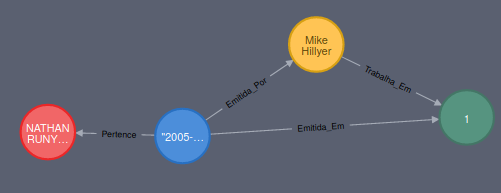
\includegraphics[width=\textwidth]{Pagamento.png}

  \caption {Representação gráfica dos nodos e Relacionamentos dos Pagamentos}

  \label {fig:Pagamento}

\end{figure}

De forma a conetar as duas partes e permitir queries mais interessantes, e mais possibilidades.Adicionou-se a relação Corresponde que coneta os nodos Pagamento e os nodos Filme, isto é, quais os pagamentos que correspondem a dado filme.

\begin{figure}[H]

  \centering

  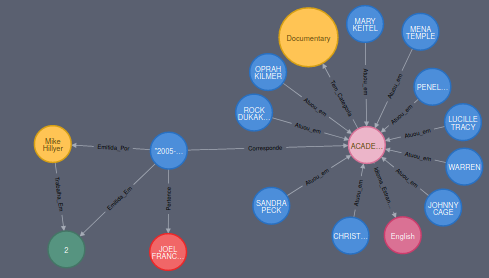
\includegraphics[width=\textwidth]{Completo.png}

  \caption {Representação Completo do grafo}

  \label {fig:Completa}

\end{figure}




\subsection{Preenchimento da Base de Dados}

O preenchimento da base de dados foi realizada tendo como base os mesmos ciclos para migrar para MongoDB e , também as mesmas queries ao MySQL(adicionando uns atributos das tabelas usadas para os Joins).Utilizando , também, Python e a Biblioteca correspondente de Neo4j.Verificando sempre se os nodos ja existem para evitar repetições.De seguida, apresenta-se as imagens com os Statments usados para evitar criações e para inserir os novos elementos para a base de dados Neo4j.Os da primeira imagem correspondem ao subgrafo relacionado com Filmes e a segunda corresponde ao subgrafo dos Pagamentos, Clientes e etc.Ainda a terceira imagem corresponde a zona que faz conexão entre os dois.Através de uma query ao MySql que junta as tabelas Rental,Payment e Inventory apresentada a seguir.

\begin{lstlisting}[language=sql,caption=Query ao MySQL para fazer a conexão entre os dois subgrafos]

SELECT payment.payment_id,rental.rental_id,inventory.film_id From 
	payment Inner JOIN rental 
		ON payment.rental_id = rental.rental_id 
		inner Join inventory 
			ON rental.inventory_id = inventory.inventory_id

\end{lstlisting}

\begin{figure}[H]

  \centering

  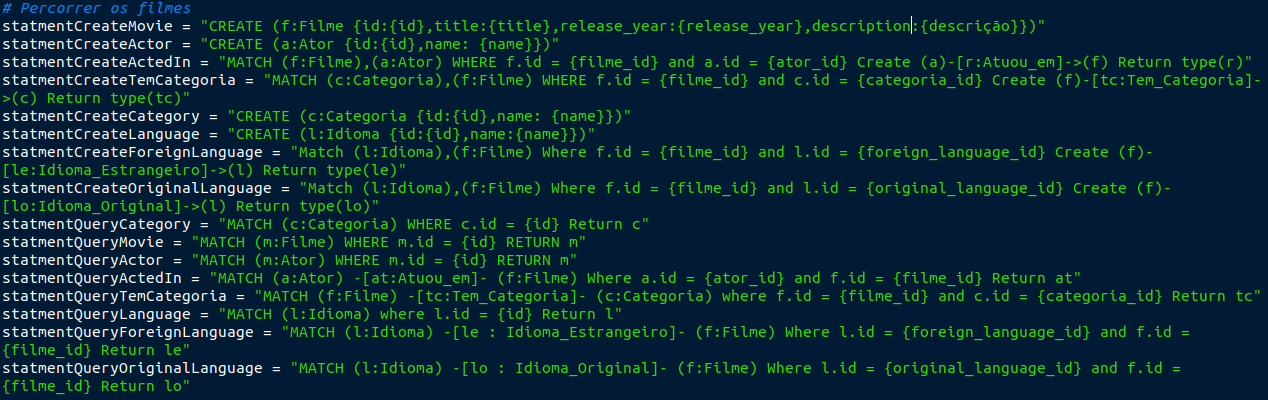
\includegraphics[width=\textwidth]{FilmesStatment.png}

  \caption {Os Statments usados no código para migrar os Filmes}

  \label {fig:FilmStatment}

\end{figure}

\begin{figure}[H]

  \centering

  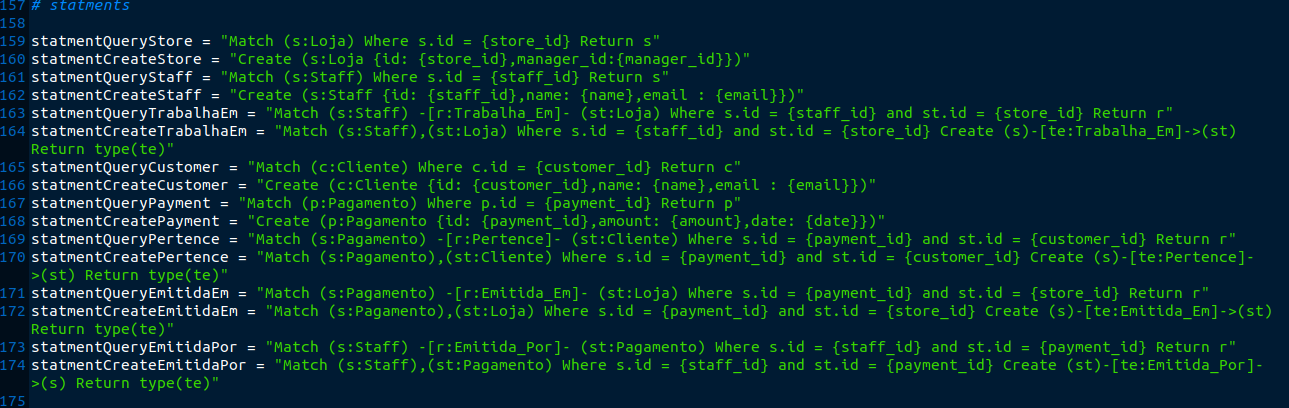
\includegraphics[width=\textwidth]{PagamentosStatment.png}

  \caption {Os Statments usados no código para migrar os Pagamentos}

  \label {fig:PagamentoStatment}

\end{figure}

\begin{figure}[H]

  \centering

  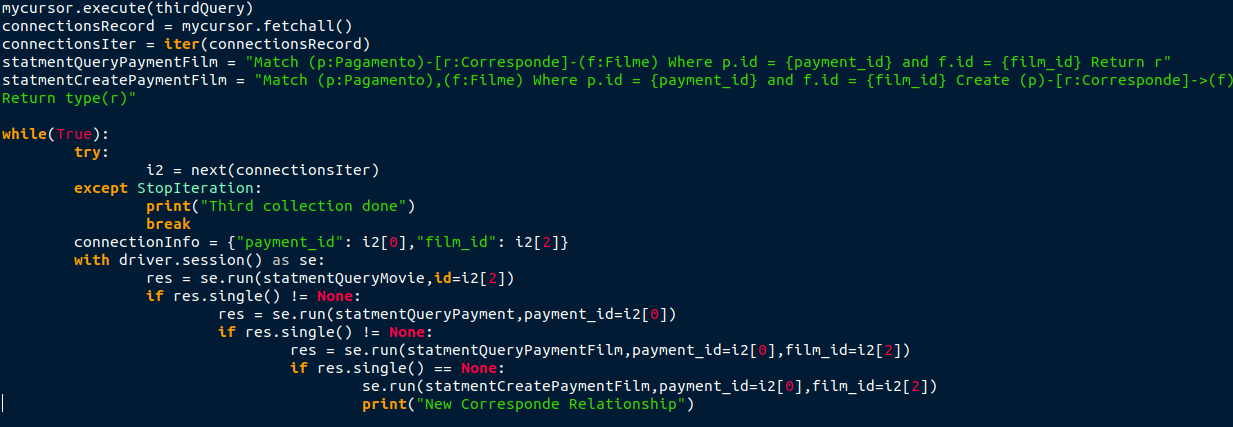
\includegraphics[width=\textwidth]{ConexaoStatment.png}

  \caption {Parte do código que relaciona os Filmes e os Pagamentos}

  \label {fig:ConexaoStatment}

\end{figure}



\subsection{Querys a Base de Dados}

A seguir apresentam-se alguns tipos de queries que podem ser feitas a base de Dados gráfica. A primeira retorna todos os filmes da Categoria Action, podendo adaptar-se para outro tipo de categorias ou para retornar todas categorias de um filme.

\begin{lstlisting}[caption=Query ao Neo4j para retornar os filmes da categoria ação]
Match (f:Filme)-[:Tem_Categoria]-(c:Categoria) 
	Where c.name = "Action" 
		Return f
\end{lstlisting}

Esta próxima permite devolver todos os atores que participaram no filme de Categoria Action.Podendo-se alterar para retornar todos os Filmes em que um ator participou etc.

\begin{lstlisting}[caption=Query ao Neo4j para retornar todos os atores que participaram em filmes de Action]
Match (f:Filme)-[r:Tem_Categoria]-(c:Categoria)
	,(a:Ator)-[:Atuou_em]-(f) 
		Where c.name = "Action" 
			Return a
\end{lstlisting}

Outra Query focada mais no lado dos Pagamentos permite retornar todos os Pagamentos realizados por um Cliente.Ainda , facilmente, poder-se-ia retornar a lista de pagamentos realizados por um Staff ou pertencentes a uma loja.

\begin{lstlisting}[caption=Query ao Neo4j para retornar todos os Pagamentos de um determindado Cliente]
Match (c:Cliente)-[:Pertence]-(p:Pagamento) 
	Where c.id = 1 
		Return p
\end{lstlisting}

Finalmente, e uma das mais úteis, utilizando a ligação que coneta as duas partes.Permite saber quais os filmes que um Cliente realizou pagamentos por.Permitindo realizar uma analise sobre os Clientes.

\begin{lstlisting}[caption=Query ao Neo4j para retornar todos os filmes que um determinar Cliente já pagou por]
Match (p:Pagamento)-[:Corresponde]-(f:Filme),
	(c:Cliente)-[:Pertence]-(p) 
		Where c.id = 1 
			Return f
\end{lstlisting}
